\documentclass{beamer}
\usepackage{hyperref}
\hypersetup{
    colorlinks=true,
    linkcolor=blue,
    filecolor=magenta,      
    urlcolor=cyan,
    pdftitle={Overleaf Example},
    pdfpagemode=FullScreen,}

\usetheme{Madrid}

% Define neutral and accent colors
\definecolor{LightGray}{RGB}{245,245,245}
\definecolor{DarkGray}{RGB}{105,105,105}
\definecolor{AccentColor}{RGB}{0,51,153}  % Demokritos Blue as an accent

% Apply the colors
\setbeamercolor{background canvas}{bg=white}
\setbeamercolor{title}{fg=DarkGray, bg=LightGray}
\setbeamercolor{frametitle}{fg=DarkGray, bg=LightGray}
\setbeamercolor{structure}{fg=AccentColor}
\setbeamercolor{item projected}{bg=AccentColor}

\title{Small-Object Detection in Remote Sensing Images and Video}
\author{Stamatios Orfanos}
\institute{University of Piraeus \hspace*{1cm} NCSR Demokritos}
\date{\today}
\titlegraphic{
\includegraphics[width=4.5cm]{Figures/University-of-Piraeus-logo-350x250.png}\hspace*{1cm}
\includegraphics[width=2cm]{Figures/demokritos-logo.png}}

\begin{document}

\begin{frame}
  \titlepage
\end{frame}

\begin{frame}
  \frametitle{Table of Contents}
  \tableofcontents
\end{frame}

\section{Introduction}
\begin{frame}[t]
  \frametitle{Introduction}
  Remote sensing imaging is a process used to gather information about objects or areas from a distance, typically using aircraft or satellites.
  Remote sensing imaging has applications across a broad spectrum of fields.
  
  \begin{columns}[T]
    \begin{column}{.4\textwidth}
      \begin{itemize}
        \item Environmental monitoring  
        \item Agriculture monitoring    
        \item Disaster management       
        \item Urban planning            
        \item Military and intelligence 
      \end{itemize}
    \end{column}
    \begin{column}{.6\textwidth}
      \begin{center}
        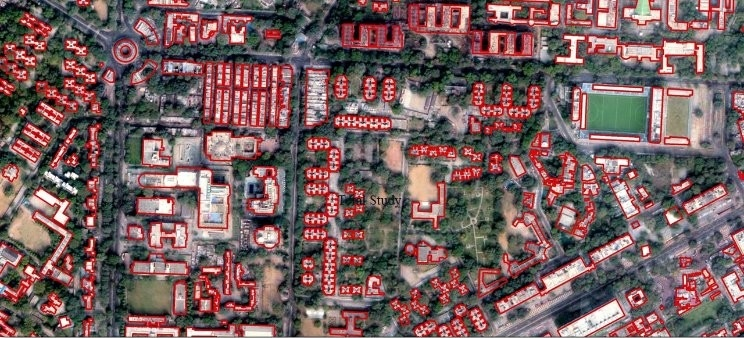
\includegraphics[width=\linewidth]{Figures/urban_planning_cropped.jpg} \\
        \small{Urban Planning}
      \end{center}
    \end{column}
  \end{columns}
\end{frame}



\begin{frame}[t]
  \frametitle{Introduction}
  In remote sensing images the objects are small fraction of the pixels of the image, qualifying this process as Small Object Detection. \\
  \vspace{0.5cm}
  Compared with large and medium objects, small objects are more difficult to detect accurately for the following reasons:
  \begin{itemize}
    \item Small objects have low resolution and insufficient features
    \item The span of object-scale is large and multiple scales coexist
    \item The examples of small objects are scarce
    \item Categories for small objects are imbalanced for the majority of datasets
  \end{itemize}
\end{frame}


\begin{frame}[t]
  \frametitle{Introduction}
  There are two ways to define small objects in the context of object detection.
  \begin{itemize}
    \item Relative size: the bounding box of a small object should cover less than 1\% of the original image
    \item Absolute size: a small object has size less than 32x32 pixels defined in MS-COCO dataset or 16x16 pixels defined in USC-GRAD-STDdb 
  \end{itemize} 

\end{frame}


\section{Data and Data Preprocessing}
\begin{frame}[t]
  \frametitle{Data and Data Preprocessing}
  The selected datasets cover a wide range of applications, from real-life scenarios to military and intelligence uses, ensuring a comprehensive evaluation 
  of the detection models.

  \begin{itemize}
    \item 1 
    % \item   \href{https://cocodataset.org/#download}{one}
    % \url{https://github.com/VisDrone/VisDrone-Dataset}
    % \url{https://www.kaggle.com/datasets/sovitrath/uav-small-object-detection-dataset}
  \end{itemize}

\end{frame}


\begin{frame}[t]
  \frametitle{COCO2017 Dataset}
  The COCO2017 dataset includes complex everyday scenes with common objects in their natural context. It features:
  \begin{itemize}
    \item Over 200,000 images
    \item 1.5 million object instances
    \item 80 object categories
  \end{itemize}
  Used for object detection, segmentation, and captioning tasks.
\end{frame}

\begin{frame}[t]
  \frametitle{Vis-Drone Dataset}
  Vis-Drone is designed for drone-based image analysis and includes:
  \begin{itemize}
    \item Around 10,209 images
    \item Images captured from various drones
    \item Focus on urban scenes and traffic monitoring
  \end{itemize}
  It is used for object detection and tracking.
\end{frame}

\begin{frame}[t]
  \frametitle{UAV-SOD Dataset}
  The UAV-SOD dataset is targeted at small object detection from aerial perspectives, featuring:
  \begin{itemize}
    \item High-resolution images
    \item Challenges due to small object scales
    \item Annotations for object detection tasks
  \end{itemize}
  Essential for research in drone-based surveillance and remote sensing.
\end{frame}

\begin{frame}[t]
  \frametitle{Data Preprocessing Steps}
  Preprocessing is crucial for normalizing data and improving model training efficiency. Steps include:
  \begin{itemize}
    \item Resizing images and annotations to a uniform size (e.g., \(600 \times 600\) pixels).
    \item Image padding to maintain aspect ratio without distortion.
    \item Annotation format standardization for consistency across datasets.
    \item Normalization of image pixel values using dataset-specific mean and standard deviation.
  \end{itemize}
\end{frame}



\section{Object Detection Metrics}
\begin{frame}
  \frametitle{Object Detection Metrics}
  % Object Detection Metrics content goes here.
\end{frame}

\section{Proposed Method}
\begin{frame}
  \frametitle{Proposed Method}
  % Proposed Method content goes here.
\end{frame}

\section{Experiments}
\begin{frame}
  \frametitle{Experiments}
  % Experiments content goes here.
\end{frame}

\section{Conclusion}
\begin{frame}
  \frametitle{Conclusion}
  % Conclusion content goes here.
\end{frame}



\end{document}
